\documentclass[12pt]{article}

\usepackage{subfigure}
\usepackage{pstricks}
\usepackage{pst-node}
\usepackage{graphicx}
\usepackage{authoraftertitle}
\usepackage[T1]{fontenc}
\usepackage{amsmath}
\usepackage{amsfonts}
\usepackage{amssymb}
\usepackage[lined,ruled,vlined,linesnumbered]{algorithm2e}
\usepackage{xspace,epsfig,url}
\usepackage{pst-plot,pstricks-add}
\usepackage{etoolbox}
\usepackage{setspace}

\AtBeginEnvironment{algorithm}{\setstretch{1}}

\SetKwFor{ForEachP}{foreach}{in parallel do}{end}

\newtheorem{theorem}{Theorem}
\newtheorem{definition}[theorem]{Definition}
%\newtheorem{remark}[theorem]{Remark}

\newenvironment{remark}
{% This is the begin code
\stepcounter{theorem}\vspace*{0.3cm}\noindent{\bf Remark} \arabic{theorem}.
}
{% This is the end code
}

\newtheorem{proposition}{Proposition}[section]
%\newtheorem{cor}[thm]{Corollary}

\newcommand{\comment}[2]{{\color{red}{\bf (#1: #2)}}}
\newcommand{\greedyAlgo}{\textsc{Greedy}}


\linespread{1.5}

\setlength{\leftmargin}{3.5cm}

\setlength{\topmargin}{2cm}

\setlength{\rightmargin}{2cm}

\newcommand{\ics}[2]{\langle #1, #2 \rangle}
%\newcommand{\ics}[2]{\frac{#1}{#2}}

\title{Algorithmic Optimization and Parallelization of Eppstein's Synchronizing Heuristic}

\author{Serta\c{c} Karahoda}

\date{}

\begin{document}

\maketitle
\thispagestyle{empty}
\vspace{1cm}

\begin{center}
Submitted to the Graduate School of Sabanc{\i} University \\
in partial fulfillment of the requirements for the degree of \\
Master of Science
\end{center}

\vspace{2cm}

\begin{center}
Sabanci University
\end{center}

\begin{center}
Augustus, 2017
\end{center}


\clearpage
$ $
\thispagestyle{empty}
\clearpage
$ $
\vspace{5cm}
\begin{center}
\copyright \hspace{0.1cm} \MyAuthor\space 2017

All Rights Reserved
\thispagestyle{empty}
\end{center}
\clearpage

\begin{center}
\large
\MyTitle
\end{center}

\begin{center}
\MyAuthor

CS, Master's Thesis, 2017

Thesis Supervisor: H\"{u}sn\"{u} Yenig\"{u}n\\
Thesis Co--Supervisor: Kamer Kaya
\end{center}

\begin{center}
Keywords: ...
\end{center}

\begin{abstract}
...
\end{abstract}
\clearpage

\begin{center}
\large
Eppstein'\i{}n S\i{}f\i{}rlama Sezgiselinin Algoritmik Eniyilemesi ve Paralelle\c{s}tirilmesi
\end{center}

\begin{center}
\MyAuthor

CS, Y\"{u}ksek Lisans Tezi, 2017

Tez Dan{\i}\c{s}man{\i}: H\"{u}sn\"{u} Yenig\"{u}n\\
Tez E\c{s}dan{\i}\c{s}man{\i}: Kamer Kaya
\end{center}

\begin{center}
Anahtar Kelimeler: ...
\end{center}

\begin{quote}
\begin{center}
{\bf \"{O}zet}
\end{center}

...

\end{quote}
\clearpage
$ $
\vspace{2cm}
\begin{center}
\textbf{Acknowledgements}
\end{center}

%I would like to state my gratitude to my supervisor, H\"{u}sn\"{u} Yenig\"{u}n for everything he has done for me, especially for his invaluable guidance, limitless support and understanding. \\
%I would like to thank Hasan Ural and Guy-Vincent Jourdan for supporting this work with precious ideas and comments. \\
%I would like to thank my family for never leaving me alone. \\
%The financial support of Sabanci University is gratefully acknowledged. \\
%I would like to thank TUBITAK for the financial support provided.


\clearpage
\tableofcontents

\clearpage 
\listoffigures

\clearpage
\listoftables

\clearpage
\listofalgorithms

\clearpage
\section{Introduction}
\label{sec:Intro}

\comment{Sertac}{Reset word'den bahsedecegim.}

\noindent
\comment{Sertac}{Intro'da FSM'den bahsedecegim.}

\noindent
\comment{Sertac}{cycle synchrop synchropl gibi algoritmalardan bahsedecegim.}

\clearpage
\section{Preliminaries}
\label{sec:Preliminaries}
FSMs are mathematical abstractions for of real word systems. When an FSM gets an input, it moves from a state to another with an output. Since synchronization sequence consider only destination state, the output is not in the scope of this work. Therefore, we can consider FSMs are as automata with simple transition function without an output.

When an {\em automaton} is complete and deterministic, it is defined by a triple $A=(S, \Sigma, \delta)$  where $S = \{1, 2, \ldots, n\}$ is a finite set of $n$ states, $\Sigma$ is a finite alphabet consisting of $p$ input symbols (or simply {\em letters}). $\delta : S \times \Sigma \rightarrow S$ is a transition function. If the automaton $A$ is at a state $s$ and if an input $x$ is applied, then $A$ moves to the state $\delta(s,x)$. Figure~\ref{fig:inv} shows an example automaton $A$ with 4 states and 2 inputs using graphical notation.\looseness=-1

\begin{figure}[ht]
\centering
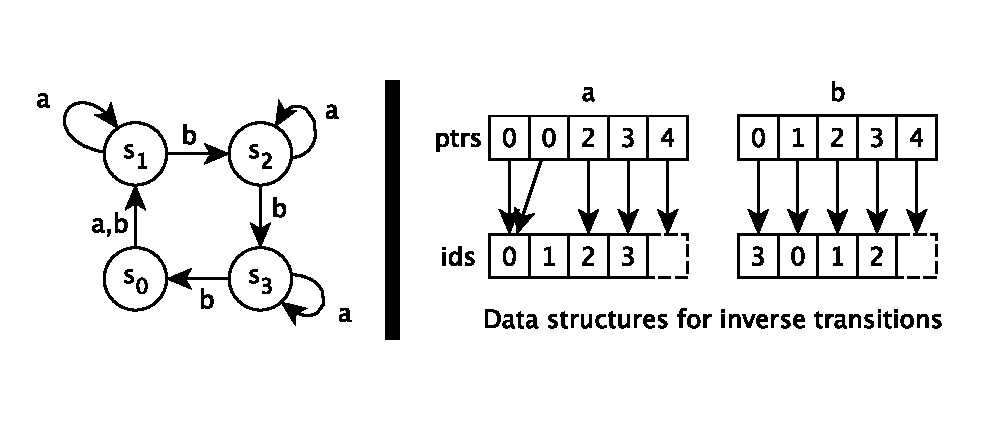
\includegraphics[width=0.7\textwidth]{figs/inverse.pdf}
\caption{A synchronizable automaton $A$~(left), and the data structures to store and process the transition function $\delta^{-1}$  in memory (right).}
\label{fig:inv}
\vspace*{-3ex}
\end{figure}

An element of the set $\Sigma^\star$ is called an {\em input sequence} (or simply {\em word}). $|w|$ denotes the length of $w$, and $\varepsilon$ expresses the empty word. Transition function $\delta$ can be extended to a set of states and to a word in the usual way. With fact $\delta(s,\varepsilon)=s$, let a word $w \in \Sigma^\star$ and a letter $x \in \Sigma$, then $\delta(s,xw) = \delta(\delta(s,x),w)$. Likewise, for a set of states $S' \subseteq S$, transition function is $\delta(S',w) = \{ \delta(s,w) | s \in S'\}$.

Inverse of the transition is also a well defined function. $\delta^{-1}(s,x)$ denotes the set of those states with a transition to state $s$ with input $x$. Formally, $\delta^{-1}(s,x) = \{ s' \in S | \delta(s',x)= s\}$.

Let $A=(S, \Sigma, \delta)$, $C \subseteq S$ and $C^{\langle 2 \rangle} = \{ \langle s_i, s_j \rangle | s_i,s_j \in C \}$ be set of multisets  with cardinality 2. For $\langle s_i, s_j \rangle \in C^{\langle 2 \rangle}$, if $s_i=s_j$ then it is called as \textit{singleton}, otherwise called as \textit{pair}. 

An automata which produced from set of pairs; ${\cal A}=(S^{\langle 2 \rangle},\Sigma,\Delta)$ is called \textit{pair automata}. For pair automata, set of inputs are same and transition function is $\Delta(\langle s_i,s_j \rangle,x) = \langle \delta(s_i,x), \delta(s_j,x)\rangle$. \comment{sertac}{pair automata icin figure cizilebilir}

Let $C \subseteq S$ and $w \in \Sigma^*$, when cardinality of $\delta(C,w)$ is 1 then $w$ is \textit{merging sequence} for $C$ and $C$ is called \textit{mergeable}. If $C=S$, $w$ is called \textit{reset word} of automaton and the automaton is synchronizable.

\clearpage
\section{Eppstein's \greedyAlgo \space Algorithm}
\label{sec:greedy}
In this section, Eppstein's \greedyAlgo \space is introduced. After that experiments and some analysis are shown. These analysis leads us to improve the speed of the algorithm.

\begin{proposition}
	\label{prop:synchronizable}
	An automaton $A=(S,\Sigma,\delta)$ is synchronizable iff for all  $s_i,s_j \in S$, there exists a merging sequence for $\{ s_i, s_j \}$.
\end{proposition}

The \greedyAlgo \space Algorithm is one of the fastest algorithm among the reset word generating heuristics in the literature. Idea of the algorithm comes from proposition \ref{prop:synchronizable}. The algorithm uses merging sequences of pairs, in fact the shortest ones, to find a short reset word. Like most of algorithms mentioned in Section \ref{sec:Intro}, \greedyAlgo \space has two main phases. At the first phase it finds the shortest merging sequences for all pairs. If there is a pair which is not mergeable, means that the automaton is not mergeable. Otherwise, the algorithm continues with second phase.

Merging sequence of pairs are stored in a function $\tau : S^{\langle 2 \rangle} \rightarrow \Sigma^\star$, which is called \textit{pairwise merging function (PMF)} for $A$. If $\{ s_i, s_j \}$ is mergeable, then $\tau(\{ s_i, s_j \})$ is the merging sequence, otherwise it is undefined. Note that PMF does not have to be unique, i.e. $\tau(\{ s_i, s_j \})$ may differ, however  $|\tau(\{ s_i, s_j \})|$ is unique. To find all shortest merging sequence, breath first search algorithm can be used. By using the inverse of transition function and starting from $\langle s_i, s_i \rangle$ singletons, all mergeable pairs and their shortest merging sequences can be found iterative. Let $p=|\Sigma|$ and $n=|s|$, at worst case the algorithm traverse all edges, i.e. $p$ letters of each $n\cdot(n-1)$ pairs and $n$ singletons should be checked. Therefore the complexity of Phase 2 is $O(pn^2)$. 

Algorithm \ref{algo:BFS} keeps track of most recent computed mergeable pairs , which is called \textit{frontier set ($F$)}. The level of frontier set refers the length of merging sequence. Since $\tau(\{ s_i, s_i \})=\epsilon$, singletons are defined as root level, level 0, of BFS algorithm. \textit{Remaining set (R)} is the set of pairs whose merging sequences are not computed yet. At each iteration of Algorithm \ref{algo:BFS} new frontier and remaining sets are computed for next level. 


\begin{algorithm}[ht]
	\label{algo:BFS}
	\caption{Computing a PMF $\tau : S^{\langle 2 \rangle} \rightarrow \Sigma^\star$}
	\SetKwInOut{Input}{input}\SetKwInOut{Output}{output}
	\Input{An automaton $A=(S,\Sigma,\delta)$}
	\Output{A PMF $\tau : S^{\langle 2 \rangle} \rightarrow \Sigma^\star$}
	
	%compute the reverse automaton ${A}^{-1} = (S,\Sigma,\delta^{-1})$ of $A$;\\
	\lForEach{singleton $\langle s,s \rangle \in S^{\langle 2 \rangle}$}{$\tau(\langle s,s \rangle) = \varepsilon$}
	\lForEach{pair $\langle s_i,s_j \rangle \in S^{\langle 2 \rangle}$}{$\tau(\langle s_i,s_j \rangle) = \mbox{\em undefined}$}
	
	$F \longleftarrow \{ \langle s,s\rangle | s \in S \}$; \tcp{all singletons of $S^{\langle 2 \rangle}$}
    $R \longleftarrow \{ \langle s_i,s_j\rangle | s_i,s_j \in S \wedge s_i \neq s_j \}$; \tcp{all pairs of $S^{\langle 2 \rangle}$}
	\While{$R$ is not empty and $F$ is not empty}
	{
		$F,R,\tau \longleftarrow \mbox{BFS\_step}(A,F,R,\tau)$;\\
	}
\end{algorithm}

\begin{proposition}
	\label{prop:merging}
	Let a pair $\langle s_i,s_j \rangle \in S^{\langle 2 \rangle}$, when a letter $x \in \Sigma$ is applied to the pair and resulting pair has merging sequence $w \in \Sigma^*$, then $x \cdot w$ is a merging sequence for the pair $\langle s_i,s_j \rangle$.
\end{proposition}

Thanks to inverse of transition function and Proposition \ref{prop:merging}, Algorithm \ref{algo:BFS-step-F2R} computes the new frontier set from the most recent frontier set. At line 3-4, algorithm searches pairs which can reach the pairs of frontier set by applying one letter. If the merging sequence of found pair is not defined, then the algorithm defines it. Since the algorithm finds the remaining set from the frontier set, it is called \textit{frontier to remaining (F2R)}. 

\begin{algorithm}[ht]
	\label{algo:BFS-step-F2R}
	\caption{{BFS\_step (F2R)}}
	
	\SetKwInOut{Input}{input}\SetKwInOut{Output}{output}
	\Input{An automaton $A=(S,\Sigma,\delta)$, the frontier $F$, the remaining set $R$, $\tau$}
	\Output{The new frontier $F'$, the new remaining set $R'$, and updated function $\tau$}
	
	$F' \longleftarrow \emptyset$;\\
	\ForEach{$ \langle s_i,s_j \rangle \in F$}
	{
		\ForEach{$x \in \Sigma$}
		{
			\ForEach{$\langle s'_i,s'_j\rangle$ such that $s'_i \in \delta^{-1}(s_i,x)$ and $s'_j \in \delta^{-1}(s_j,x)$}
			{
				\If(\tcp*[h]{$\langle s'_i,s'_j\rangle \in R$}){$\tau(\langle s'_i,s'_j\rangle)$ is undefined}
				{
					$\tau(\langle s'_i,s'_j\rangle) \longleftarrow x \tau(\langle s_i,s_j \rangle)$;\\
					$F' = F' \cup \{ \langle s'_i,s'_j\rangle  \} $;\\
				}
			}
		}
	}
	let $R'$ be $R \setminus F'$;
\end{algorithm}

When first phase is completed, Algorithm \ref{algo:greedy} checks the automata is synchronizable or not in $O(n^2)$ (line 2,3). After that it finds reset word iterative. it initialize the \textit{set of active states (C)} as set of all states and the reset word as empty word. At each iteration it selects the shortest merging sequence of all active pairs; appends it to reset word; finally updates the set of active states with applying the selected merging sequence. This operation repeats until only one active state left. At each iteration, merging sequence is applied, so the cardinality of $C$ decreases. Therefore iteration repeats at most $n$ times. At line 7 apply minimum operation among active pairs which is $O(n^2)$. Line 8 takes constant time. the complexity of computation line 9 is $O(n^?)$. Thus Phase 2 takes $O(n^?)$ and Algorithm \ref{algo:greedy} requires $O(pn^2 + n^?)$ time. At Section \ref{sec:greedy-analysis}, bottleneck of the algorithm is introduced with experimental analysis.

\comment{sertac}{complexity $O(n^3)$ mu demeliyiz yoksa $O(n^4)$ mu? interediate phaseden bahsetmeli miyiz?}

\begin{algorithm}[ht]
	\label{algo:greedy}
	\caption{Eppstein's \textsc{Greedy} Algorithm}
	
	\SetKwInOut{Input}{input}\SetKwInOut{Output}{output}
	\Input{An automaton $A=(S,\Sigma,\delta)$}
	\Output{A reset word $\Gamma$ for $A$ (or fail if $A$ is not synchronizable)}
	
	%{--- Phase 1 ---}
	compute a PMF $\tau$ using Algorithm~\ref{algo:BFS}\;
	\If{there exists a pair $\langle s_i,s_j \rangle$ such that  $\tau(\langle s_i,s_j \rangle)$ is undefined}
	{
		report that $A$ is not synchronizable and exit;	
	}

	
	%{--- Phase 2 ---}
	$C = S$; \tcp{$C$ will keep track of the current set of states}
	$\Gamma = \varepsilon$; \tcp{$\Gamma$ is the synchronizing sequence to be constructed}
	
	\While(\tcp*[h]{we have two or more states yet to be merged}){$|C| > 1$}
	{
		find a pair $\langle s_i,s_j \rangle \in C^{\langle 2 \rangle}$ 
		with minimum $|\tau(\langle s_i,s_j \rangle)|$ among all pairs 
		in $C^{\langle 2 \rangle}$;\\
		
		
		$\Gamma = \Gamma \; \tau(\langle s_i,s_j \rangle)$;\\
		$C = \delta(C,\tau(\langle s_i,s_j \rangle))$;
	}
\end{algorithm}


\subsection{Analysis on \greedyAlgo}
\label{sec:greedy-analysis}


In Section \ref{sec:greedy}, \greedyAlgo \space Algorithm introduced and its two phase structure is explained. Complexity of PMF construction, first phase, is $O(pn^2)$ and complexity of \greedyAlgo \space is based on Phase 2 of the algorithm which has $O(n^?)$ time complexity. To analyze the algorithm, we perform experiments on 100 randomly generated automata for each  $p \in \{2, 8, 32, 128\}$ letters and  $n \in \{2000, 4000, 8000\}$ states. In addition to these automata we also use Cerny automata \cite{cerny} for $n \in \{2000, 4000, 8000\}$ states. Total 1200 randomly generated automata, in Table \ref{table:phase-comparison}, shows that the opposite of complexity calculation; first phase dominates the execution time of the algorithm.

\begin{table}[ht]
	\begin{center}
	\scalebox{0.8}{
		\begin{tabular}{r|rrr|rrr|rrr}
		&\multicolumn{3}{|c}{$n = 2000$}&\multicolumn{3}{|c}{$n = 4000$}&\multicolumn{3}{|c}{$n = 8000$}\\
		$p$ & $t_{PMF}$ & $t_{ALL}$ & $\frac{t_{PMF}}{t_{ALL}}$ & $t_{PMF}$ & $t_{ALL}$ & $\frac{t_{PMF}}{t_{ALL}}$ & $t_{PMF}$ & $t_{ALL}$ & $\frac{t_{PMF}}{t_{ALL}}$\\\hline
			2		& 0.172	& 0.185	& 0.929	& 1.184		& 1.240		& 0.954	& 5.899		& 6.325		& 0.933 \\
			8		& 0.504	& 0.517	& 0.975	& 2.709		& 2.768		& 0.978	& 14.289	& 14.721	& 0.971 \\
			32		& 2.113	& 2.126	& 0.994	& 9.925		& 9.986		& 0.994	& 51.783	& 52.233	& 0.991 \\
			128		& 9.126	& 9.140	& 0.999	& 40.356	& 40.418	& 0.998	& 193.548	& 193.982	& 0.998 \\
			cerny	& 0.096	& 4.836	& 0.020	& 1.026		& 42.771	& 0.024	& 5.584		& 797.692	& 0.007\\
		\end{tabular}
		}
	\end{center}
	\caption{Sequential PMF construction time ($t_{PMF}$), and overall time ($t_{ALL}$) in seconds}
	\label{table:phase-comparison}
\end{table}

\comment{sertac}{Phase 2 kac iteration oldu deneyi eklenebilir}

To understand the behavior of the algorithm, we extend our experiments by analyzing the structure of PMF. While computing time complexity of the algorithm, we take the length of merging sequence is at most $n^2$. However, Table \ref{table:levels} shows that $n^2$ is loose bound for the length of merging sequence.For instance, when automata with 8000 states and 128 letters are considered, the length of merging sequence in PMFs is at most 3, not 64000000. Another observation, Phase 2 tends to pick smaller length of merging sequences. For example, when we take automata with 8000 states and 2 letters, The longest merging sequence in PMF has length 16.9 and Phase uses only merging sequences with length 12.1 and less, on average. It means merging sequences of almost \%30 of nodes are not necessarily computed (see Figure \ref{fig:nodes-at-levels}).

\begin{table}[ht]
\center
\begin{tabular}{r|rrr|rrr|rrr}
 & \multicolumn{3}{c|}{n=2000} & \multicolumn{3}{c|}{n=4000} & \multicolumn{3}{c}{n=8000} \\
p &  $h_{PMF}$ &  $h_{max}$ &  $h_{mean}$ &  $h_{PMF}$ &  $h_{max}$ &  $h_{mean}$ &  $h_{PMF}$ &  $h_{max}$ &  $h_{mean}$ \\ \hline
 2 &  14.2 &  10.0 &  1.9 &  15.5 &  11.2 &  1.9 &  16.9 &  12.1 &  1.9 \\
 8 &  5.0 &  4.0 &  1.3 &  6.0 &  4.2 &  1.3 &  6.0 &  4.6 &  1.3 \\
 32 &  3.1 &  2.7 &  1.1 &  4.0 &  2.9 &  1.1 &  4.0 &  3.0 &  1.1 \\
 128 &  3.0 &  2.0 &  1.0 &  3.0 &  2.0 &  1.0 &  3.0 &  2.1 &  1.0
\end{tabular}
\caption{The length of longest merging sequence in PMF($h_{PMF}$) constructed in Phase 1; maximum ($h_{max}$), and average ($h_{mean}$) lengths for merging sequences, used in Phase 2 of \greedyAlgo. \comment{sertac}{cerny deneyleri}}
\label{table:levels}
\end{table}

\begin{figure}[ht]
	\centering
	\subfigure[$n = 2000$]{
		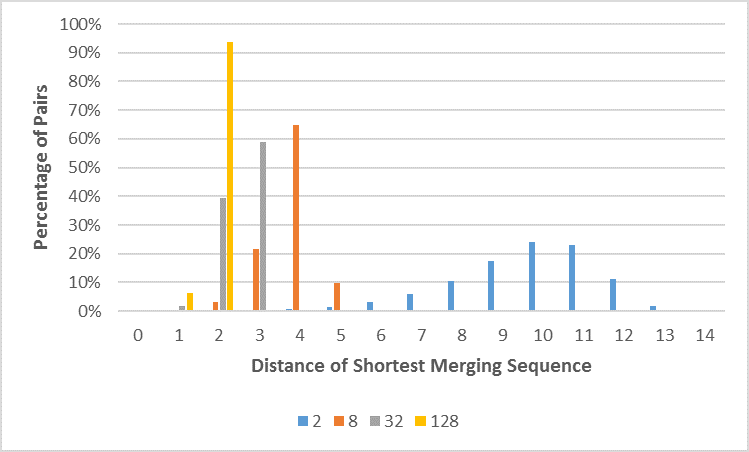
\includegraphics[width=0.45\textwidth]{figs/node_2000.png}
	}
	\subfigure[$n = 4000$]{
		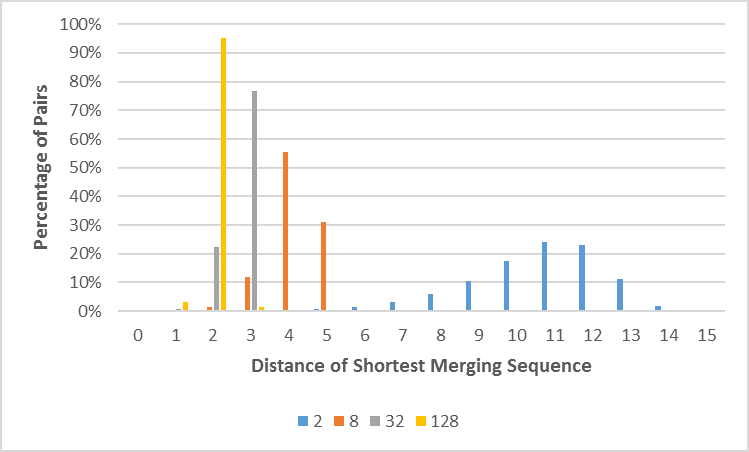
\includegraphics[width=0.45\textwidth]{figs/node_4000.png}
	}
	\subfigure[$n = 8000$]{
		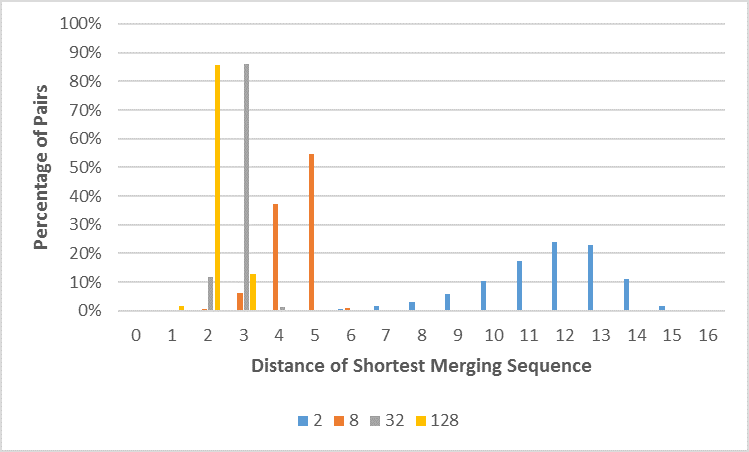
\includegraphics[width=0.45\textwidth]{figs/node_8000.png}
	}
	\caption{The percentage of nodes at each level in PMF \comment{sertac}{distance yerine length yazmak lazim. Daha okunabilir ve diger graphlerle uyumlu bir halini yapmak icin graphlerin exceldeki hallerini bulmam lazim}}
	\label{fig:nodes-at-levels}
	\vspace*{-2.5ex}
\end{figure}


With the help of experiments, we observe that execution time of PMF construction phase dominates \greedyAlgo \space Algorithm. We also notice that all information from first phase is not used in second phase. Therefore we focused on parallelization of PMF construction, which is explained in Section \ref{sec:parallel}. Also some algorithmic improvements to prevent unnecessary computations in first phase are introduced in Section \ref{sec:speedup}.

\clearpage
\section{Parallelization on \greedyAlgo}
\label{sec:parallel}

Section \ref{sec:greedy-analysis} conclude that PMF construction is the bottleneck of \greedyAlgo . To minimize the cost of PMF construction, we implement various algorithms. In this section parallel algorithms are introduced.

Algorithm \ref{algo:BFS} is a BFS algorithm which starts from singletons and searches the merging sequences of all pairs. Length of the merging sequence for a pair represents level of the pair in BFS tree. Since the merging sequence of singletons is $\epsilon$, The algorithm initially sets singletons as level 0 nodes. To find $k^{th}$ level nodes, Algorithm \ref{algo:BFS-step-F2R} gets $k-1^{st}$ level as frontier set. The cost of processing each pair in frontier set, depends on inverse of transition function $\delta^{-1}$. Likewise the cost of each iteration depends on the number of pair in frontier set. Therefore the cost of each task and number of task in each iteration vary. In CPU parallelization, we use OpenMP and dynamic scheduling to handle tasks. 

\comment{sertac}{BFS icin ornek figure cizilebilir}

\subsection{Frontier to Remaining in Parallel}
\label{sec:BFS-F2R-parallel}

While finding pair from $k^{th}$ level (setting $k^{th}$ level as next frontier set $F'$) the algorithm have to ensure that all pairs from $k-1^{st}$ level are found. Likewise, the algorithm shall process all pairs from $i^{th}$ level(using $i^{th}$ level as frontier set $F$) before process a pair from $i+1^{st}$ level. Since sequential algorithm for PMF construction process one pair at a time, a simple queue is enough to schedule processing of pairs. The algorithm stores singletons, level 0 nodes and picks the next processed node from the beginning of the queue. When a new pair is found, the algorithm pushes the pair at the end of queue. Using queue is a flawless method to maintain the dependency between tasks. Implementing parallel version of the algorithm is not easy as sequential version. Each thread shall process pairs from same level to preserve task dependency. Using queue is not enough and a barrier mechanism is needed.

\begin{algorithm}[ht]
	\label{algo:BFS-step-F2R-Parallel}
	\caption{BFS\_step\_F2R (in parallel)}
	
	\SetKwInOut{Input}{input}\SetKwInOut{Output}{output}
	\Input{An automaton $A=(S,\Sigma,\delta)$, the frontier $F$, the remaining set $R$, $\tau$}
	\Output{The new frontier $F'$, the new remaining set $R'$, and updated function $\tau$}
	
	\lForEach{thread $t$}{
		$F'_t \longleftarrow \emptyset$
	}
	\ForEachP{$\langle s_i,s_j\rangle \in F$}
	{
		\ForEach{$x \in \Sigma$}
		{
			\ForEach{$\langle s'_i,s'_j\rangle$ where $s'_i \in \delta^{-1}(s_i,x)$ and $s'_j \in \delta^{-1}(s_j,x)$}
			{
				\If(\tcp*[h]{$\langle s'_i,s'_j\rangle \in R$}){$\tau({\langle s'_i,s'_j\rangle})$ is undefined}
				{
					$\tau(\langle s'_i,s'_j\rangle) \longleftarrow x \tau(\langle s_i,s_j\rangle )$;\\
					$F'_t = F'_t \cup \{ \langle s'_i,s'_j \rangle  \} $;\\
				}
			}
		}
	}
	$F' \longleftarrow \emptyset$;\\
	\lForEach{thread t}{
		$F' = F' \cup F'_t$
	}
	let $R'$ be $R \setminus F'$;
\end{algorithm}

In implementation of Algorithm \ref{algo:BFS-step-F2R-Parallel}, we separate $F$ and $F'$. Threads partition all pairs in $F$. When the algorithm finds a new pair, it pushes to new frontier set. Since pushing an item to a set is not atomic operation, we also change the process of pushing a pair to the next frontier set. The easiest way is putting the operation to a critical region. However this is not a time efficient method. So we implement a lock-free mechanism, instead of global $F'$, each thread stores a local $F'$. When all pairs from $F$ are processed, a thread(master thread) merges local $F'$s in a sequential manner. Lock free mechanism comes with a drawback. When two threads find same pair $\langle s'_i,s'_j\rangle$, at line 6 of Algorithm \ref{algo:BFS-step-F2R-Parallel}, at the same time, then both of them pushes the same pair to $F'$ and duplicate data is occurred. In CPU parallelization, our experimental observations shows that at most thousandth of $|F'|$ pairs are duplicate. Since duplicate pair does not effect the correctness of the algorithm, we avoid the time cost of eliminating duplicate pair by using processing extra pair whose time cost is negligible compered to earlier. Except the redundant computation, duplicate pair is also obstacle to implement $R'$ (line 8). In parallel implementation, Algorithm  \ref{algo:BFS} can check only $F$ (line 5).  

\subsection{Remaining to Frontier}
\label{sec:BFS-R2F-parallel}

Processing the frontier set $F$ to set the next frontier set $F'$ , like in \ref{algo:BFS-step-F2R} and \ref{algo:BFS-step-F2R-Parallel}, is most natural and common way for a BFS algorithm. Another approach is processing the remaining set $R$, to find $F'$, we called as \textit{remaining to frontier (R2F)}. The main difference R2F uses transition function $\delta$ as edges, compared to F2R uses $\delta^{-1}$. Thanks to Proposition \ref{prop:merging}, Algorithm \ref{algo:BFS-step-R2F-Parallel} searches all pairs $\langle s_i,s_j\rangle \in R$ and applies all possible letters $x \in \Sigma$. If the algorithm finds a merging sequence $\delta(\langle s_i,s_j\rangle, x) = w$ (lines 4-6), then it sets $\tau = (\langle s_i,s_j\rangle) = x \cdot w$ (lines 7-9), otherwise the pair remains in the next remaining set $R'$ (lines 10, 11). Like in Algorithm \ref{algo:BFS-step-F2R-Parallel}, Algorithm \ref{algo:BFS-step-R2F-Parallel} also uses local sets. Each thread $t$ uses own local the next remaining set $R'_t$ for lock-free parallelization. Note that, each thread process different pair $\langle s_i,s_j\rangle$, hence there is no duplicate pair in $R'$; Algorithm \ref{algo:BFS} can uses $R$ and the algorithm iterates one less compared to F2R. However R2F algorithm process a pair at each iteration until merging sequence of that pair is found.

\begin{algorithm}[ht]
	\label{algo:BFS-step-R2F-Parallel}
	\caption{BFS\_step\_R2F (in parallel)}
	
	\SetKwInOut{Input}{input}\SetKwInOut{Output}{output}
	\Input{An automaton $A=(S,\Sigma,\delta)$, the frontier $F$, the remaining set $R$, $\tau$}
	\Output{The new frontier $F'$, the new remaining set $R'$, and updated function $\tau$}
	
		\lForEach{thread t}{$R'_t \longleftarrow \emptyset$}
		\ForEachP{$\langle s_i,s_j\rangle \in R$}
		{
			$connected  \longleftarrow $ {\bf false};\\
			\ForEach{$x \in \Sigma$}
			{
				$\langle s'_i, s'_j \rangle \longleftarrow \langle \delta(s_i,x),\delta(s_j,x) \rangle$; \\ 

				\If(\tcp*[h]{$\langle s'_i,s'_j\rangle \in F$}){$\tau(\langle s'_i, s'_j\rangle)$ is defined}
				{
					$\tau(\langle s_i, s_j\rangle) \longleftarrow x \tau(\langle s'_i, s'_j\rangle)$;\\
					$connected  \longleftarrow $ {\bf true};\\
					{\bf break};\\
				}
			}
			\If{not $connected$}
			{
					$R'_t = R'_t \cup \{ \langle s_i, s_j\rangle \} $;\\
			}
		}
		$R' \longleftarrow \emptyset$;\\
		\lForEach{thread t}{
			$R' = R' \cup R'_t$
		}
		let $F'$ be $R \setminus R'$;
\end{algorithm}


\subsection{Hybrid Approach}
\label{sec:BFS-Hybrid-parallel}




\clearpage
\section{Speeding up the Fastest}
\label{sec:speedup}
\comment{sertac}{Makalenin ismi guzel oldugu icin onu yazdim ama baska isim koymak gerekir mi emin olamadim.}



\clearpage
\section{Conclusion and Future Works}
\label{sec:conclusion}

\comment{sertac}{speeding up the fastest lookahead implementation'da hesapladigimiz merging sequencelari kaydetmiyoruz. onlari kaydederek giden bir algoritma daha hizli olabilir belki.}

\comment{sertac}{algoritmalar icin web interface}

\clearpage
\bibliographystyle{plain}
\bibliography{thesis}

\end{document}


